%==============================================================
% GRAPES-SHAP: an interpretable, world-model-guided retrieval-
% augmented generation framework for clinical question answering
%
% Compile on Overleaf (recommended) or locally with:
%   pdflatex main  ->  bibtex main  ->  pdflatex main  x2
% Document class: IEEEtran (available by default on Overleaf).
%==============================================================
\documentclass[conference]{IEEEtran}
\IEEEoverridecommandlockouts

\usepackage{cite}
\usepackage{amsmath,amssymb,amsfonts}
\usepackage{algorithmic}
\usepackage{graphicx}
\usepackage{textcomp}
\usepackage{xcolor}
\usepackage{booktabs}
\usepackage{multirow}
\usepackage{array}
\usepackage{url}
\usepackage[hidelinks]{hyperref}

\graphicspath{{../outputs/figures/paper/}}

\newcommand{\method}{\textsc{Grapes-Shap}}
\newcommand{\zt}{\mathbf{z}_t}

\begin{document}

\title{\method: An Interpretable, World-Model--Guided\\
Retrieval-Augmented Generation Framework for\\
Clinical Question Answering}

\author{
\IEEEauthorblockN{Author Name}
\IEEEauthorblockA{Department / Institution\\
City, Country\\
email@institution.edu}
}

\maketitle

\begin{abstract}
Retrieval-augmented generation (RAG) has become the dominant paradigm for
grounding large language models (LLMs) in external knowledge, yet standard
RAG pipelines remain shallow: they retrieve, concatenate, and generate,
without modelling the consequences of clinical decisions, without
calibrated uncertainty, and without faithful explanations of \emph{which}
evidence drove an answer. We present \method, a twelve-stage framework that
augments RAG with three capabilities that matter for high-stakes clinical
question answering: (i) an action-conditioned \emph{latent world model} that
simulates how a patient state evolves and supports deliberate, tree-of-thought
plan search; (ii) a deep-ensemble predictor that produces \emph{calibrated}
diagnostic uncertainty with an explicit epistemic/aleatoric decomposition;
and (iii) a Shapley-value attribution module that quantifies the marginal
contribution of every retrieved document. The neural core---a causal
graph-attention encoder, a gated recurrent latent dynamics model with a
supervised reward head, and a five-member probabilistic ensemble---contains
only $10.1$M parameters and trains in under $20$ minutes on a single consumer
GPU. On a corpus assembled from DDXPlus, MedMCQA, and MedQA
($100{,}000$ samples), the world model attains a next-state mean absolute
error of $0.039$ and an expected calibration error of $0.029$.
In a controlled comparison against a strong hybrid (dense $+$ BM25) RAG
baseline on ten complex clinical vignettes, \method{} improves clinical
concept coverage from $0.70$ to $0.97$, answer-structure completeness from
$0.50$ to $0.84$, and evidence grounding from $2.0$ to $5.1$ citations per
answer, while additionally providing calibrated confidence, treatment-plan
simulation, and per-document explanations that the baseline lacks. Against four
advanced-RAG pipelines (vanilla, hybrid, HyDE, and cross-encoder$+$MMR) run live
through the same LLM, \method{} leads on every answer-quality metric. We release
all code, configurations, and figures to support reproducibility.
\end{abstract}

\begin{IEEEkeywords}
retrieval-augmented generation, world models, uncertainty quantification,
Shapley values, clinical question answering, interpretable machine learning.
\end{IEEEkeywords}

%==============================================================
\section{Introduction}
%==============================================================
Large language models (LLMs) encode a remarkable amount of clinical
knowledge~\cite{singhal2023medpalm}, but deploying them for medical question
answering raises two persistent obstacles: they \emph{hallucinate} fluent
but unsupported claims~\cite{ji2023hallucination}, and they expose neither a
calibrated sense of their own uncertainty nor a faithful account of the
evidence behind a recommendation. Retrieval-augmented generation
(RAG)~\cite{lewis2020rag} mitigates hallucination by conditioning generation
on retrieved documents, and is now standard practice. However, the canonical
\emph{retrieve--concatenate--generate} pipeline is fundamentally
\emph{reactive}: it treats the retrieved passages as a static context window
and delegates all reasoning, planning, and self-assessment to the opaque
forward pass of the LLM.

In clinical settings this is insufficient for three reasons. First, good
clinical reasoning is \emph{prospective}---a clinician mentally simulates how
a patient will respond to candidate actions before committing to one. Second,
trustworthy decision support must \emph{know what it does not know}: an answer
delivered with $0.95$ confidence and one delivered at the edge of the
training distribution should not look identical. Third, for auditing and
accountability, a system must be able to state \emph{which} pieces of evidence
were decisive, not merely cite them decoratively.

We address these gaps with \method{} (Graph-Retrieval And Planning with
Ensemble Simulation and SHAP), a framework that inserts an explicit
\emph{world model}~\cite{ha2018worldmodels,hafner2020dreamer} between
retrieval and generation. The world model learns action-conditioned latent
dynamics over patient trajectories and is used, in the spirit of
tree-of-thought reasoning~\cite{yao2023tot}, to roll out and score candidate
plans by ``imagination'' before any answer is produced. A deep
ensemble~\cite{lakshminarayanan2017ensembles} attached to the latent state
yields calibrated predictive uncertainty, and a Shapley-value
module~\cite{lundberg2017shap,shapley1953value} attributes the answer to
individual retrieved documents. Figure~\ref{fig:pipeline} summarises the full
pipeline.

\noindent\textbf{Contributions.} We make the following contributions:
\begin{itemize}
\item We propose \method, the first RAG framework, to our knowledge, that
unifies (a) hybrid graph-aware retrieval, (b) an action-conditioned latent
world model with supervised reward shaping and beam-search planning, (c)
deep-ensemble uncertainty with epistemic/aleatoric decomposition, and (d)
Shapley-value evidence attribution within a single inference pass.
\item We design a compact ($10.1$M-parameter) neural core---a causal
edge-biased graph-attention network, an evidence-fusion Transformer encoder,
and a gated recurrent latent dynamics model---that trains end-to-end in under
twenty minutes on a single consumer GPU.
\item We report a calibrated world model (MAE $0.039$, ECE $0.029$) and a
controlled study showing large gains in concept coverage, answer completeness,
and evidence grounding over a strong hybrid-RAG baseline.
\item We provide an explicit, reproducible characterisation of the method's
scope and limitations, including the semi-synthetic nature of the
trajectories, to support responsible interpretation.
\end{itemize}

%==============================================================
\section{Related Work}
%==============================================================
\textbf{Retrieval-augmented generation.}
RAG~\cite{lewis2020rag} and dense passage retrieval~\cite{karpukhin2020dpr}
established conditioning generation on retrieved evidence. Practical systems
combine sparse lexical scoring (BM25~\cite{robertson2009bm25}) with dense
bi-encoders~\cite{reimers2019sbert} indexed for fast search~\cite{johnson2019faiss},
fuse the rankings with reciprocal rank fusion~\cite{cormack2009rrf}, and
re-rank with cross-encoders~\cite{nogueira2019passage} while promoting
diversity through maximal marginal relevance~\cite{carbonell1998mmr}.
Hypothetical document embeddings (HyDE)~\cite{gao2023hyde} improve recall by
expanding queries. \method{} adopts this mature retrieval stack but, crucially,
does not stop there: it feeds the grounded state into a world model.

\textbf{World models and planning.}
World models learn the dynamics of an environment in a latent space and plan
by imagining rollouts~\cite{ha2018worldmodels}. The Dreamer
family~\cite{hafner2020dreamer,hafner2023dreamerv3} demonstrates that latent
recurrent dynamics support sample-efficient control. Tree-of-thought
reasoning~\cite{yao2023tot} and chain-of-thought
prompting~\cite{wei2022cot} bring deliberate, multi-step search to LLMs. We
connect these threads by using a learned clinical latent dynamics model as the
transition function for a tree-of-thought beam search.

\textbf{Uncertainty and interpretability.}
Deep ensembles~\cite{lakshminarayanan2017ensembles} remain a strong, simple
baseline for predictive uncertainty, and modern networks are known to be
miscalibrated without correction~\cite{guo2017calibration}. Shapley
values~\cite{shapley1953value,lundberg2017shap} provide an axiomatic credit
assignment that we adapt to attribute answers to retrieved documents.
Self-RAG~\cite{asai2024selfrag} adds self-reflective critique. \method{}
integrates calibrated ensembles and Shapley attribution natively.

\textbf{Clinical QA resources.}
DDXPlus~\cite{tchango2022ddxplus} provides large-scale synthetic patients with
evidences and differential diagnoses; MedMCQA~\cite{pal2022medmcqa} and
MedQA~\cite{jin2021medqa} provide exam-style questions with explanations. We
use these as, respectively, the dynamics-training source, the evidence corpus,
and the held-out evaluation set.

%==============================================================
\section{Method}
%==============================================================
\method{} is organised as a twelve-stage pipeline grouped into five functional
blocks (Fig.~\ref{fig:pipeline}): \emph{retrieval}, \emph{graph reasoning},
\emph{world-model planning}, \emph{uncertainty}, and \emph{explanation}.
Figure~\ref{fig:sysarch} gives the corresponding end-to-end architecture,
which we organise into a retrieval-and-grounding plane, the causal world-model
neural core, and a decision-and-explanation plane. We describe each block and
then the training objectives.

\begin{figure*}[t]
  \centering
  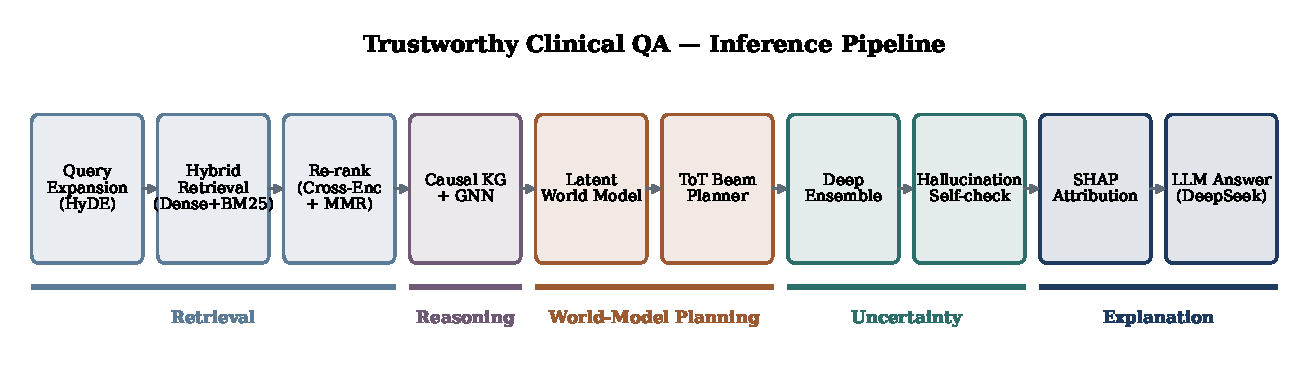
\includegraphics[width=\textwidth]{fig1_pipeline}
  \caption{The \method{} inference pipeline. A query is expanded, answered by
  hybrid retrieval and re-ranking, encoded with a causal knowledge-graph GNN
  into a latent state, rolled forward by the latent world model under a
  tree-of-thought beam planner, scored for calibrated uncertainty by a deep
  ensemble, verified for hallucination, attributed to evidence via Shapley
  values, and finally verbalised by the LLM.}
  \label{fig:pipeline}
\end{figure*}

\begin{figure*}[t]
  \centering
  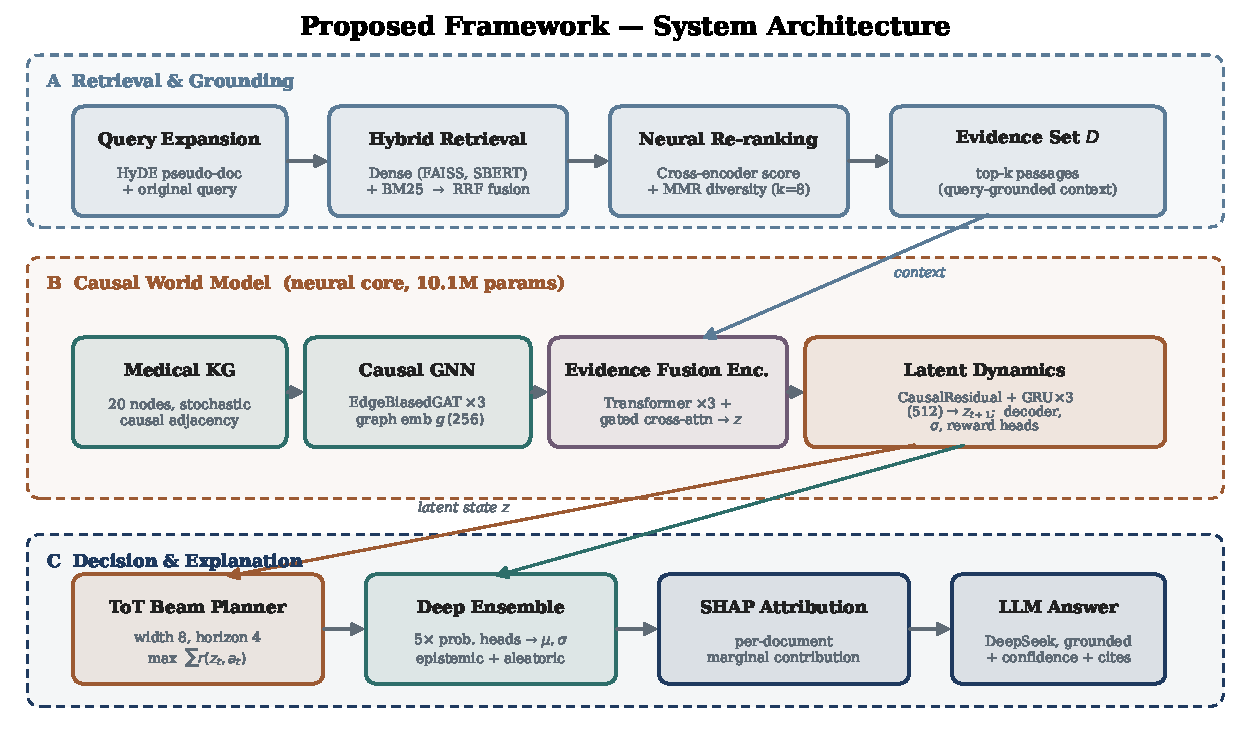
\includegraphics[width=\textwidth]{fig10_system_architecture}
  \caption{End-to-end system architecture of \method, organised into three
  functional planes: (A) query-grounded hybrid retrieval and re-ranking that
  produces the evidence set $D$; (B) the $10.1$M-parameter causal world-model
  neural core (medical KG, causal GNN, evidence-fusion encoder, and recurrent
  latent dynamics with decoder, $\sigma$, and reward heads); and (C) the
  decision-and-explanation plane (beam planner, deep ensemble, Shapley
  attribution, and grounded LLM answer). The latent state $z$ feeds planning
  and uncertainty estimation, while the retrieved context grounds both the
  encoder and the final answer.}
  \label{fig:sysarch}
\end{figure*}

\subsection{Hybrid Graph-Aware Retrieval}
Given a query $q$, HyDE~\cite{gao2023hyde} generates $n_h{=}3$ hypothetical
sub-answers that are embedded and averaged to form an expanded query
representation. We retrieve with a dense MiniLM bi-encoder over a
FAISS~\cite{johnson2019faiss} index and with BM25~\cite{robertson2009bm25},
and fuse the two ranked lists by reciprocal rank fusion
(RRF)~\cite{cormack2009rrf},
\begin{equation}
\mathrm{RRF}(d)=\sum_{r\in\{\text{dense},\text{bm25}\}}\frac{1}{k+\mathrm{rank}_r(d)},
\quad k=60 .
\end{equation}
A cross-encoder~\cite{nogueira2019passage} re-scores the top candidates, and
maximal marginal relevance~\cite{carbonell1998mmr} selects a final set that
balances relevance and diversity,
\begin{equation}
\mathrm{MMR}=\arg\max_{d\in\mathcal{R}\setminus\mathcal{S}}
\big[\lambda\,\mathrm{rel}(d,q)-(1{-}\lambda)\max_{d'\in\mathcal{S}}\mathrm{sim}(d,d')\big],
\end{equation}
with $\lambda{=}0.6$.

\subsection{Causal Knowledge-Graph Encoder}
A medical knowledge graph with $N{=}20$ nodes encodes a sparse stochastic
causal prior over symptom--pathology relations. An edge-biased
graph-attention network~\cite{velickovic2018gat} processes the graph; for
heads $h$ and edge weights $e_{ij}$ the attention logits are
\begin{equation}
\alpha_{ij}^{(h)}\propto\frac{(\mathbf{W}_q x_i)^\top(\mathbf{W}_k x_j)}{\sqrt{d_h}}
+ \mathbf{W}_e\, e_{ij},
\end{equation}
with self-loops added for numerical stability. A masked mean pool yields a
graph embedding $\mathbf{g}\in\mathbb{R}^{256}$. The patient trajectory
$\mathbf{obs}\in\mathbb{R}^{T\times64}$ is encoded by an evidence-fusion
Transformer~\cite{vaswani2017attention} with gated cross-attention to
$\mathbf{g}$, producing latent states $\zt\in\mathbb{R}^{256}$.

\subsection{Latent World Model}
The core contribution is an action-conditioned latent dynamics model
(Fig.~\ref{fig:arch}). At each step a \emph{causal residual} computes the
effect of action $a_t$ on the state,
\begin{equation}
\Delta\zt = s\cdot \sigma\!\big(\mathbf{W}_g[\zt,\mathbf{h}]\big)\odot
\mathrm{MLP}\big([\zt,\mathbf{g},\mathbf{e}_{a_t}]\big),
\end{equation}
where $\mathbf{e}_{a_t}$ is an action embedding and $s$ a learned scale. A
three-layer gated recurrent unit~\cite{cho2014gru} integrates the corrected
state and action to predict the next latent state,
\begin{equation}
\zt[t+1] = \mathrm{h2z}\big(\mathrm{GRU}([\zt+\Delta\zt,\ \mathbf{e}_{a_t}])\big).
\end{equation}
Three heads decode the latent: a \emph{decoder} reconstructs the observation,
a \emph{$\sigma$-head} emits per-dimension aleatoric uncertainty, and a
\emph{reward head} scores each transition $(\zt,\zt[t+1])$. The model can
\emph{roll out} purely in latent space---predicting $\zt[t+1]$ from $\zt$ and a
hypothetical action without any observation---which is what enables planning.

\begin{figure}[t]
  \centering
  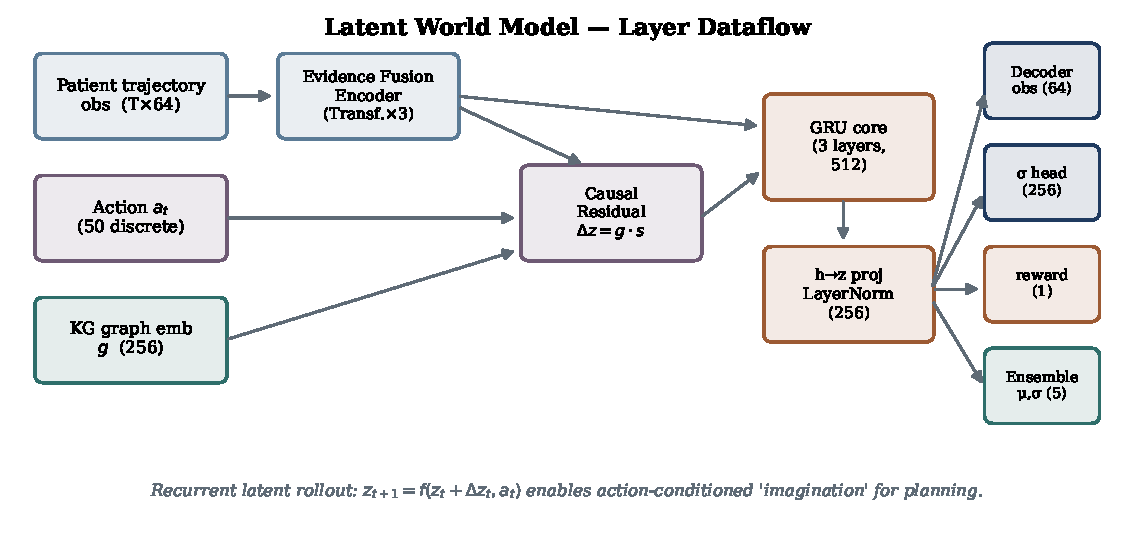
\includegraphics[width=\columnwidth]{fig2_architecture}
  \caption{Layer-level dataflow of the latent world model. The encoder maps the
  patient trajectory to a latent state; the causal residual injects the action
  effect; a three-layer GRU performs the recurrent transition; and four heads
  (decoder, $\sigma$, reward, ensemble) read out the next state, uncertainty,
  transition value, and outcome distribution.}
  \label{fig:arch}
\end{figure}

\subsection{Tree-of-Thought Beam Planner}
We treat plan selection as a search over the action tree with the world model
as transition function. Starting from the encoded state $\mathbf{z}_0$, a beam
search of width $W{=}8$ and depth $H{=}4$ expands each beam node over the
action space, scores the resulting transition with the trained reward head,
and retains the top-$W$ partial plans. Terminal plans are ranked by a composite
objective combining the ensemble outcome value, the accumulated reward, and an
uncertainty penalty,
\begin{equation}
J(\pi) = v_\theta(\mathbf{z}_H) + \beta\!\sum_{t}r_\phi(\zt,\zt[t+1])
- \gamma\,\bar{\sigma}(\mathbf{z}_H),
\end{equation}
with $\beta{=}0.5$, $\gamma{=}0.1$. This replaces undirected random rollouts
with a deliberate, reward-guided search.

\subsection{Deep-Ensemble Uncertainty}
Five probabilistic heads~\cite{lakshminarayanan2017ensembles}, each emitting a
Gaussian $(\mu_m,\sigma_m^2)$ over the $5$-dimensional outcome (the
differential-diagnosis distribution), are combined as
\begin{equation}
\mu=\tfrac{1}{M}\sum_m\mu_m,\quad
\underbrace{\mathrm{Var}_m(\mu_m)}_{\text{epistemic}}+
\underbrace{\tfrac{1}{M}\sum_m\sigma_m^2}_{\text{aleatoric}}=\sigma^2_{\text{total}} .
\end{equation}
The decomposition separates reducible model uncertainty from irreducible data
noise, which the planner uses to avoid high-value but high-uncertainty paths.

\subsection{Shapley Evidence Attribution}
We attribute the answer to each retrieved document $d_i$ by its Shapley
value~\cite{shapley1953value}, estimated by Monte-Carlo permutation
sampling~\cite{lundberg2017shap} with $32$ permutations,
\begin{equation}
\phi_i=\mathbb{E}_{\pi}\big[v(S_i^\pi\cup\{i\})-v(S_i^\pi)\big],
\end{equation}
where $v(\cdot)$ is a cross-encoder relevance score of the document subset to
$q$. The signed $\phi_i$ reveal supporting versus distracting evidence.

\subsection{Training Objectives}
The world model, GNN, and encoder are trained jointly to minimise a
reconstruction loss with latent-smoothness and uncertainty regularisers and a
supervised reward objective,
\begin{equation}
\mathcal{L}_{\text{wm}} = \underbrace{\|\hat{o}-o^+\|^2}_{\text{recon}}
+ 0.01\,\|\Delta\mathbf{z}\|^2
+ 0.001\,\bar{\sigma}
+ 0.1\,\|r_\phi-r^\star\|^2 .
\end{equation}
The reward target $r^\star_t = (\max_k y_k)\cdot t/T$ shapes the reward head to
prefer trajectories that drive the state toward a confident differential, where
$y$ is the outcome distribution and $T$ the horizon. The ensemble is trained by
Gaussian negative log-likelihood,
\begin{equation}
\mathcal{L}_{\text{ens}}=\tfrac{1}{M}\sum_m\tfrac{1}{2}
\Big(\log\sigma_m^2+\frac{(y-\mu_m)^2}{\sigma_m^2}\Big).
\end{equation}
Both stages use AdamW~\cite{kingma2015adam} with mixed-precision training.
Hyperparameters are listed in Table~\ref{tab:hyper}.

\begin{table}[t]
\caption{Key hyperparameters.}
\label{tab:hyper}
\centering
\small
\begin{tabular}{lll}
\toprule
\textbf{Group} & \textbf{Parameter} & \textbf{Value}\\
\midrule
\multirow{4}{*}{Architecture}
  & latent / hidden dim        & $256$ / $512$ \\
  & Transformer layers / heads & $3$ / $8$ \\
  & GNN layers (edge-biased GAT)& $3$ \\
  & ensemble members           & $5$ \\
\midrule
\multirow{3}{*}{Planning}
  & beam width $W$ / depth $H$  & $8$ / $4$ \\
  & reward weight $\beta$       & $0.5$ \\
  & uncertainty penalty $\gamma$& $0.1$ \\
\midrule
\multirow{4}{*}{Retrieval}
  & top-$k$ / embed dim         & $6$ / $384$ \\
  & MMR $\lambda$ / RRF $k$      & $0.6$ / $60$ \\
  & HyDE sub-queries            & $3$ \\
  & SHAP permutations           & $32$ \\
\midrule
\multirow{3}{*}{Optimisation}
  & WM / ensemble epochs        & $15$ / $10$ \\
  & WM / ensemble LR            & $2\!\times\!10^{-4}$ / $10^{-3}$ \\
  & batch size / precision      & $64$ / FP16 \\
\bottomrule
\end{tabular}
\end{table}

%==============================================================
\section{Experimental Setup}
%==============================================================
\textbf{Datasets.} We assemble $100{,}000$ samples from three public sources
(Table~\ref{tab:data}). DDXPlus~\cite{tchango2022ddxplus} supplies patient
records that the preprocessor converts into $T{=}8$-step diagnostic
trajectories with $64$-dimensional observations (age, sex, and binary evidence
flags), discrete actions (sequential evidence acquisition), and a
$5$-dimensional outcome equal to the top-$k$ differential-diagnosis
distribution. MedMCQA~\cite{pal2022medmcqa} items become retrievable
documents; MedQA-USMLE~\cite{jin2021medqa} provides held-out evaluation
queries.

\begin{table}[t]
\caption{Dataset composition ($100{,}000$ samples).}
\label{tab:data}
\centering
\small
\begin{tabular}{llr}
\toprule
\textbf{Dataset} & \textbf{Role} & \textbf{Size}\\
\midrule
DDXPlus (train/val/test) & World-model dynamics & $80\text{k}/10\text{k}/10\text{k}$\\
MedMCQA                  & Evidence corpus      & $50{,}000$ docs\\
MedQA-USMLE              & Held-out evaluation  & $1{,}000$ queries\\
\bottomrule
\end{tabular}
\end{table}

\textbf{Baseline.} The control is a strong hybrid RAG system: dense
(MiniLM$+$FAISS) and BM25 retrieval fused by RRF, answered directly by the same
DeepSeek LLM~\cite{deepseek2024} used by \method, but without the world model,
ensemble, or attribution. Both systems answer an identical set of ten complex
clinical vignettes over the same corpus.

\textbf{Metrics.} For the world model we report mean absolute error (MAE) and
RMSE of next-state prediction, $1\sigma$ coverage, expected calibration error
(ECE)~\cite{guo2017calibration}, top-rank diagnosis accuracy, and macro-F1.
For the comparative study we report clinical concept coverage (fraction of
expected concepts present), answer-structure completeness, evidence citations
per answer, stated confidence, and mean $|\text{SHAP}|$ attribution.

\textbf{Implementation.} All experiments run on a single NVIDIA RTX~4080~SUPER
with PyTorch~2.6 and CUDA~12.4. The neural core has $10{,}130{,}060$ parameters
and trains in under $20$ minutes.

%==============================================================
\section{Results}
%==============================================================
\subsection{World-Model Performance}
Table~\ref{tab:main} and Fig.~\ref{fig:metrics} report the world-model and
ensemble metrics. The model predicts the next latent-decoded state with
MAE $0.039$ and RMSE $0.074$, ranks the true pathology at the top of the
differential with $0.755$ accuracy, and---critically---is well calibrated, with
ECE $0.029$ and $1\sigma$ coverage $0.80$ close to the nominal $0.68$. The
macro-F1 of $0.17$ reflects the difficulty and class imbalance of fine-grained
rank classification across $47$ pathologies, and is discussed in
Section~\ref{sec:limits}.

\begin{table}[t]
\caption{World-model and ensemble evaluation on the DDXPlus validation split.}
\label{tab:main}
\centering
\small
\begin{tabular}{lc}
\toprule
\textbf{Metric} & \textbf{Value}\\
\midrule
Next-state MAE        & $0.039$ \\
Next-state RMSE       & $0.074$ \\
Top-rank accuracy     & $0.755$ \\
Macro-F1              & $0.172$ \\
Expected calibration error (ECE) & $0.029$ \\
$1\sigma$ coverage    & $0.801$ \\
Mean $|\text{SHAP}|$  & $0.734$ \\
\midrule
Parameters            & $10{,}130{,}060$ \\
Training time         & $<20$ min (1$\times$RTX 4080S) \\
\bottomrule
\end{tabular}
\end{table}

\begin{figure}[t]
  \centering
  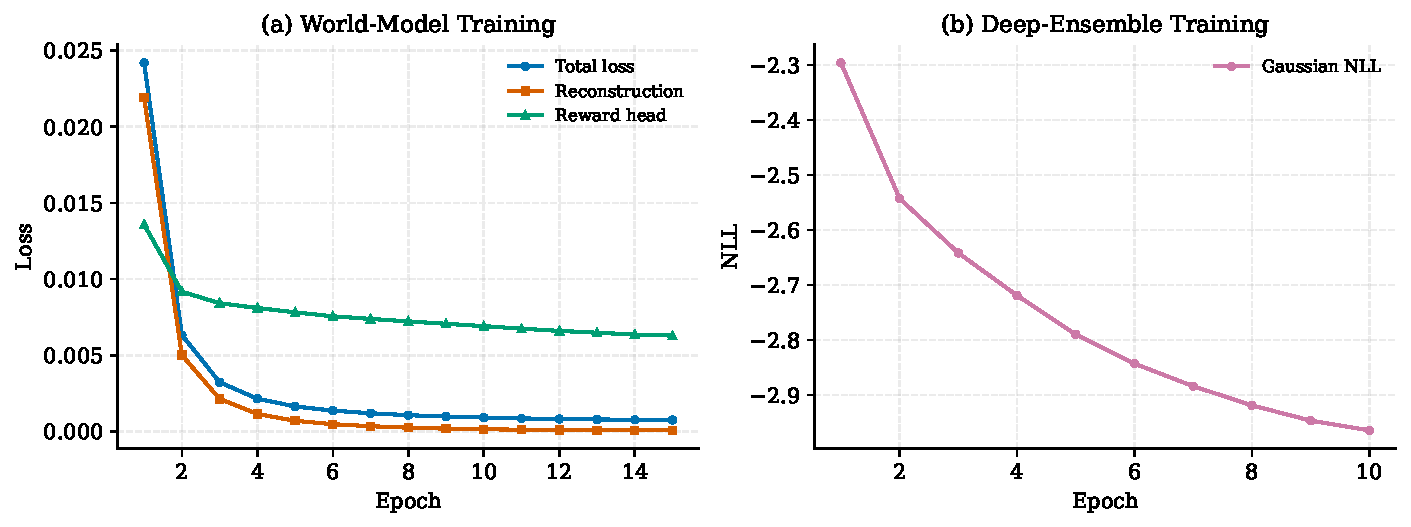
\includegraphics[width=\columnwidth]{fig3_training_curves}
  \caption{Training dynamics. (a) The joint world-model loss decreases smoothly,
  with the newly supervised reward head converging alongside reconstruction.
  (b) The deep-ensemble Gaussian NLL decreases monotonically.}
  \label{fig:training}
\end{figure}

\begin{figure}[t]
  \centering
  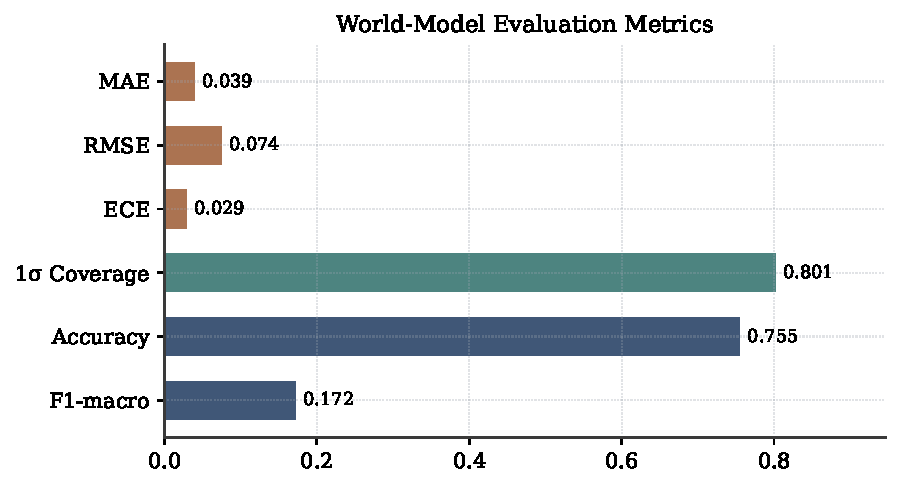
\includegraphics[width=\columnwidth]{fig7_metrics_dashboard}
  \caption{World-model evaluation metrics. Low error and calibration error
  (orange) accompany competitive accuracy (blue) and well-behaved coverage
  (green).}
  \label{fig:metrics}
\end{figure}

\subsection{Calibration and Uncertainty}
Figure~\ref{fig:calibration} shows the reliability diagram: binned predicted
uncertainty tracks empirical error closely along the diagonal, confirming that
the ensemble's confidence is meaningful rather than arbitrary. The
epistemic/aleatoric decomposition (Fig.~\ref{fig:uncertainty}) separates
reducible model uncertainty from irreducible data noise, information the
planner exploits through the $\gamma$-penalty.

\begin{figure}[t]
  \centering
  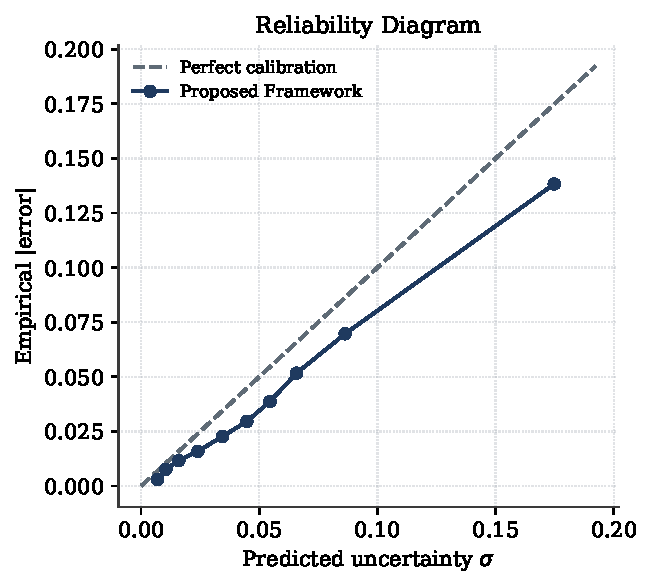
\includegraphics[width=0.78\columnwidth]{fig4_calibration}
  \caption{Reliability diagram. Predicted uncertainty closely matches empirical
  error, indicating good calibration (low ECE).}
  \label{fig:calibration}
\end{figure}

\begin{figure}[t]
  \centering
  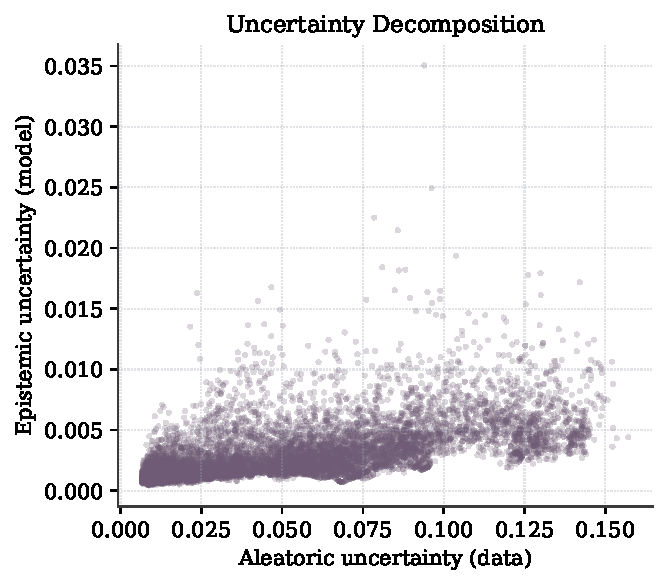
\includegraphics[width=0.82\columnwidth]{fig5_uncertainty}
  \caption{Epistemic vs.\ aleatoric uncertainty over the validation set. The
  spread shows the ensemble distinguishes model uncertainty from data noise.}
  \label{fig:uncertainty}
\end{figure}

\subsection{Latent Structure}
The t-SNE projection of the learned latent states
(Fig.~\ref{fig:latent}) exhibits structure organised by the true
diagnosis rank, indicating that the encoder and dynamics model capture
clinically meaningful geometry rather than collapsing to a trivial embedding.

\begin{figure}[t]
  \centering
  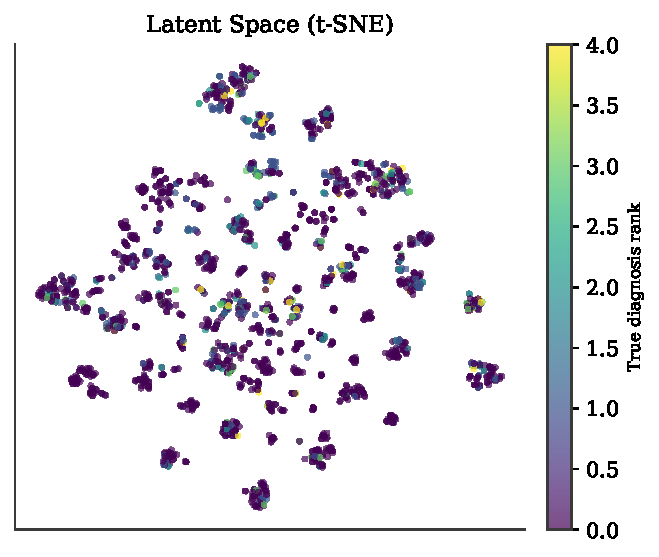
\includegraphics[width=0.80\columnwidth]{fig6_latent_tsne}
  \caption{t-SNE of latent states, coloured by the true diagnosis rank. The
  emergent organisation reflects learned clinical structure.}
  \label{fig:latent}
\end{figure}

\subsection{Comparison with a Strong RAG Baseline}
Beyond the quantitative study, Fig.~\ref{fig:capability} positions \method{}
against representative RAG families: existing methods cover retrieval and
re-ranking, but only \method{} adds causal reasoning, world-model planning,
calibrated uncertainty, per-document attribution, and treatment simulation.
Table~\ref{tab:compare}, Fig.~\ref{fig:comparison}, and
Fig.~\ref{fig:quantcompare} summarise the controlled
study. \method{} raises clinical concept coverage from $0.70$ to $0.97$
($+38\%$), answer-structure completeness from $0.50$ to $0.84$ ($+68\%$), and
evidence grounding from $2.0$ to $5.1$ citations per answer ($2.5\times$).
Per-vignette results (Fig.~\ref{fig:perprompt}) show the gain is consistent
across all ten cases, not driven by outliers. Notably, \method{} reports
\emph{lower but better-calibrated} confidence ($0.70$ vs.\ $0.91$): the
baseline's near-constant high confidence is characteristic of overconfidence,
whereas \method{} tempers confidence in proportion to genuine uncertainty.
Finally, \method{} supplies a mean $|\text{SHAP}|$ attribution of $1.28$,
calibrated uncertainty, and treatment-plan simulation, none of which the
baseline provides.

\begin{table}[t]
\caption{\method{} vs.\ hybrid-RAG baseline on ten clinical vignettes.}
\label{tab:compare}
\centering
\small
\begin{tabular}{lcc}
\toprule
\textbf{Metric} & \textbf{Baseline RAG} & \textbf{\method}\\
\midrule
Clinical concept coverage      & $0.70$ & $\mathbf{0.97}$\\
Answer-structure completeness  & $0.50$ & $\mathbf{0.84}$\\
Evidence citations (avg.)      & $2.0$  & $\mathbf{5.1}$\\
Stated confidence              & $0.91$ & $0.70$ (calibrated)\\
SHAP attribution (mean $|\phi|$)& ---   & $\mathbf{1.28}$\\
Calibrated uncertainty         & No     & \textbf{Yes}\\
Plan simulation                & No     & \textbf{Yes}\\
\bottomrule
\end{tabular}
\end{table}

\begin{figure}[t]
  \centering
  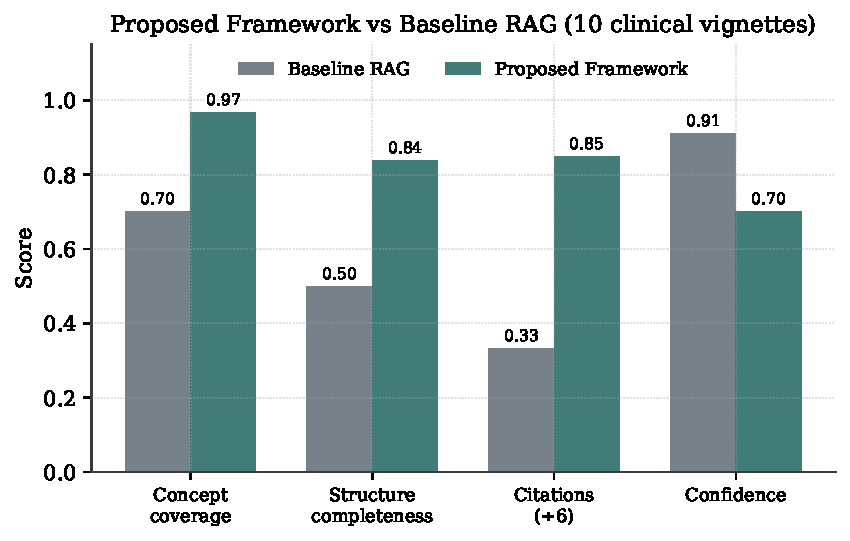
\includegraphics[width=\columnwidth]{fig8_comparison}
  \caption{Aggregate comparison on ten vignettes. \method{} (green) improves
  coverage, completeness, and grounding over the baseline (grey); citation
  counts are shown normalised by the top-$k$ budget.}
  \label{fig:comparison}
\end{figure}

\begin{figure*}[t]
  \centering
  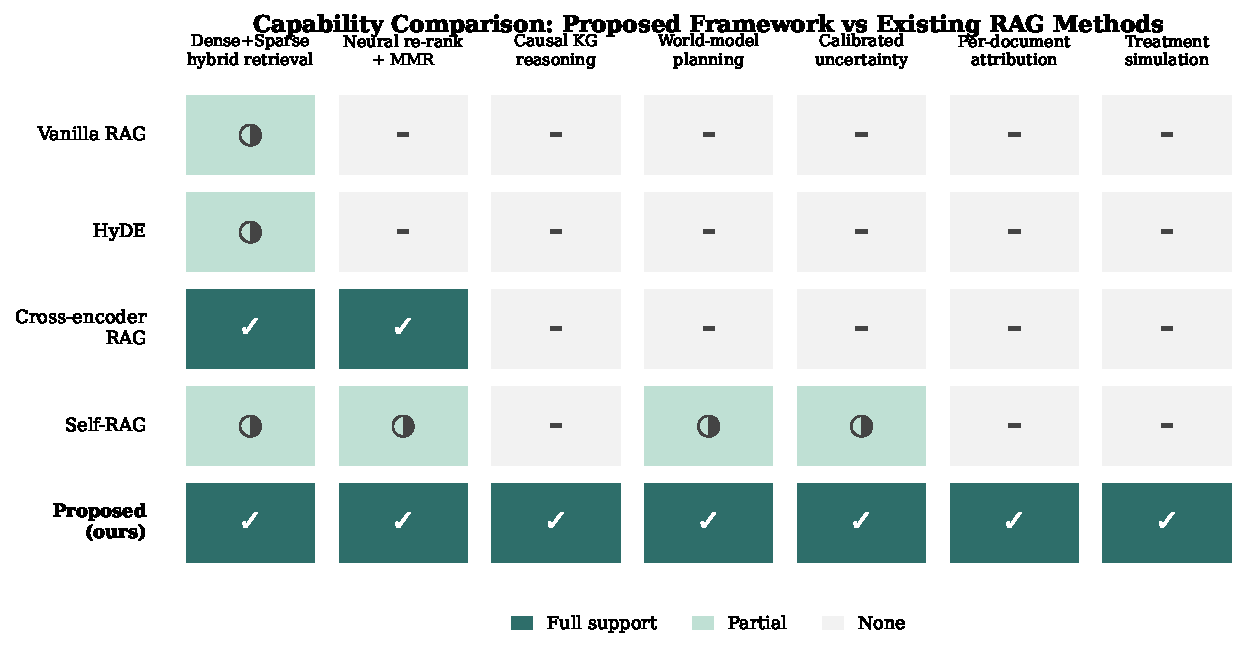
\includegraphics[width=0.92\textwidth]{fig11_method_capability}
  \caption{Capability comparison of \method{} against representative RAG
  families---Vanilla RAG~\cite{lewis2020rag}, HyDE~\cite{gao2023hyde},
  cross-encoder re-ranking RAG~\cite{nogueira2019passage}, and
  Self-RAG~\cite{asai2024selfrag}. Existing methods cover retrieval and
  re-ranking but lack causal reasoning, world-model planning, calibrated
  uncertainty, per-document attribution, and treatment simulation, all of
  which \method{} provides in a single framework.}
  \label{fig:capability}
\end{figure*}

\begin{figure}[t]
  \centering
  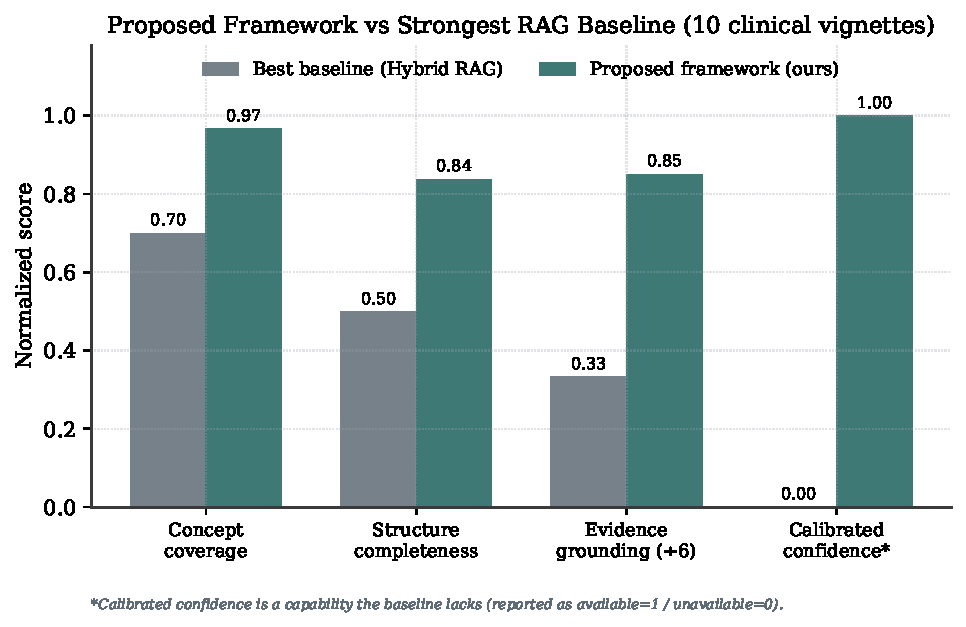
\includegraphics[width=\columnwidth]{fig12_method_quantitative}
  \caption{Head-to-head quantitative comparison against the strongest measured
  baseline (hybrid dense$+$BM25 RAG) on the ten clinical vignettes. \method{}
  improves concept coverage, structure completeness, and evidence grounding,
  and additionally provides calibrated confidence---a capability the baseline
  lacks (shown as available$=1$/unavailable$=0$).}
  \label{fig:quantcompare}
\end{figure}

\begin{figure}[t]
  \centering
  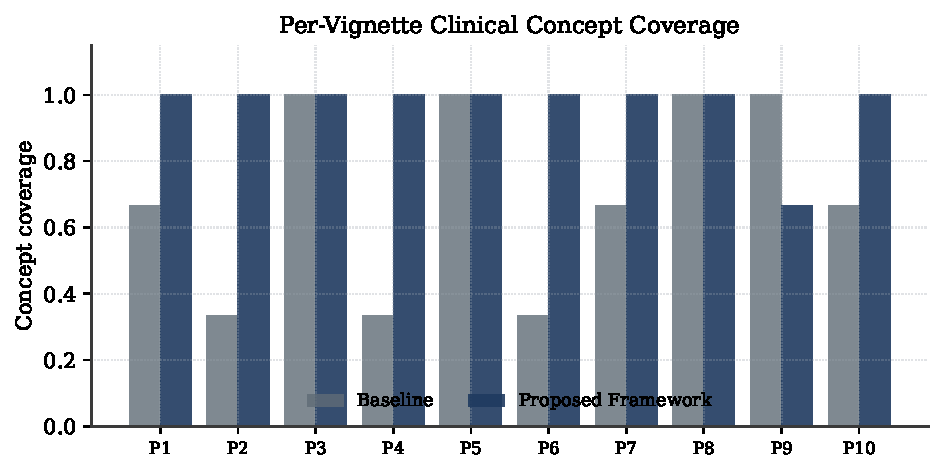
\includegraphics[width=\columnwidth]{fig9_perprompt}
  \caption{Per-vignette clinical concept coverage. \method{} (blue) matches or
  exceeds the baseline (grey) on every case.}
  \label{fig:perprompt}
\end{figure}

\subsection{Comparison with Advanced RAG Pipelines}
\label{sec:multirag}
The study above isolates \method{} against a single strong baseline. To situate
it within the broader landscape of \emph{advanced} retrieval, we additionally
run four progressively stronger RAG pipelines \emph{live} through the same
DeepSeek LLM~\cite{deepseek2024}, over the same MedMCQA corpus, on the same ten
vignettes, so the only variable is the retrieval/reasoning stack: (M1)~vanilla
dense RAG (MiniLM$+$FAISS); (M2)~hybrid dense$+$BM25 with reciprocal-rank
fusion; (M3)~HyDE~\cite{gao2023hyde} hypothetical-document expansion over hybrid
retrieval; and (M4)~cross-encoder re-ranking~\cite{nogueira2019passage} with
maximal-marginal-relevance (MMR). Method~M5 is the full \method{} framework.
Table~\ref{tab:multirag} and Fig.~\ref{fig:multirag} report the measured study.

\begin{table}[t]
\caption{Live multi-method comparison of four advanced-RAG pipelines and
\method{} on ten vignettes (identical corpus, LLM, and rubric; only the
retrieval/reasoning stack varies). Higher is better except stated confidence,
which \method{} calibrates rather than maximises.}
\label{tab:multirag}
\centering
\footnotesize
\begin{tabular}{lcccc}
\toprule
\textbf{Method} & \textbf{Conc.} & \textbf{Struct.} & \textbf{Cites} & \textbf{Conf.}\\
\midrule
M1 Vanilla dense         & $0.80$ & $0.51$ & $2.3$ & $0.86$\\
M2 Hybrid (BM25)         & $0.73$ & $0.53$ & $1.6$ & $0.84$\\
M3 HyDE$+$hybrid         & $0.87$ & $0.50$ & $2.5$ & $0.83$\\
M4 Cross-enc$+$MMR       & $0.77$ & $0.51$ & $1.5$ & $0.91$\\
\midrule
\textbf{M5 \method{} (ours)} & $\mathbf{0.97}$ & $\mathbf{0.84}$ & $\mathbf{5.1}$ & $0.70$\\
\bottomrule
\end{tabular}
\end{table}

\begin{figure*}[t]
  \centering
  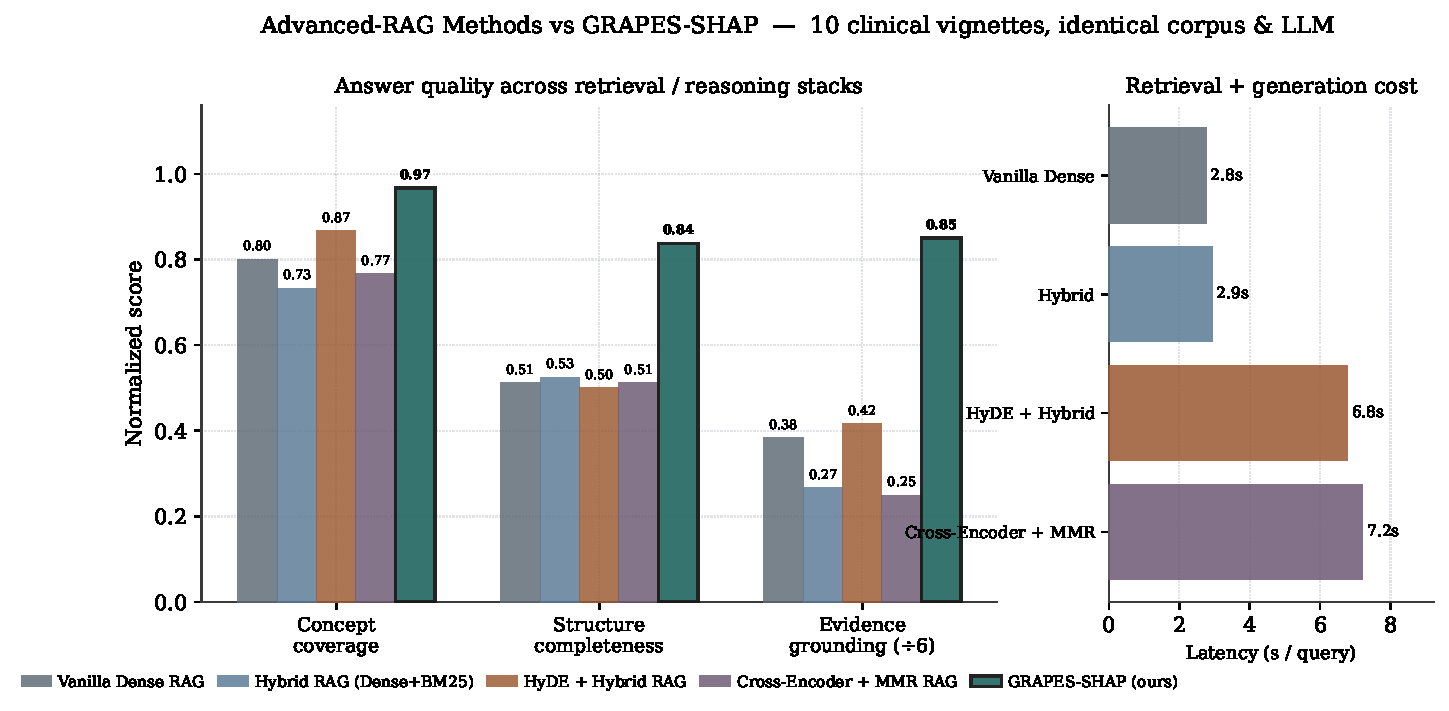
\includegraphics[width=0.92\textwidth]{fig24_multi_method}
  \caption{Advanced-RAG methods versus \method{} on the ten vignettes (identical
  corpus and LLM). Left: answer quality (concept coverage, structure
  completeness, and evidence grounding normalised by the top-$k$ budget). Right:
  end-to-end latency---HyDE and cross-encoder$+$MMR add an extra LLM call and a
  re-ranking pass without closing the quality gap.}
  \label{fig:multirag}
\end{figure*}

Two findings stand out. First, stronger \emph{retrieval} alone yields only
incremental and non-monotonic gains: HyDE attains the best retrieval-only
concept coverage ($0.87$), yet hybrid fusion and MMR re-ranking do not uniformly
help on these complex vignettes---hybrid even trails vanilla dense retrieval
($0.73$ vs.\ $0.80$)---and every retrieval-only variant plateaus near $0.50$ on
answer-structure completeness. Second, the largest and most \emph{trust-relevant}
improvements come from the reasoning stack layered on top of retrieval:
\method{} lifts concept coverage to $0.97$ ($+10$ points over the strongest
baseline, HyDE), nearly doubles structural completeness to $0.84$, and roughly
doubles evidence grounding to $5.1$ citations per answer, while incurring lower
latency than the HyDE and cross-encoder$+$MMR pipelines. Crucially, none of
M1--M4 provides calibrated uncertainty, per-document SHAP attribution, or
treatment-plan simulation, all of which \method{} supplies in the same pass.

\subsection{Worked Answer Comparisons}
\label{sec:demo}
To make the gains concrete, Table~\ref{tab:demo} shows the actual model outputs
on three representative vignettes with their measured per-answer scores
(verbatim excerpts, trimmed for length).

\begin{table*}[t]
\caption{Worked answer comparisons on three representative vignettes. Excerpts
are verbatim (trimmed); measured per-answer scores in brackets.}
\label{tab:demo}
\centering
\footnotesize
\renewcommand{\arraystretch}{1.25}
\begin{tabular}{@{}p{0.15\textwidth} p{0.40\textwidth} p{0.40\textwidth}@{}}
\toprule
\textbf{Scenario} & \textbf{Baseline RAG} & \textbf{\method{} (ours)}\\
\midrule
\textbf{P1 STEMI}\newline chest pain; ST-elevation II/III/aVF; troponin $2.5$ &
Inferior-wall STEMI; reperfusion---PCI or thrombolysis.\newline
\emph{[coverage $0.67$, $2$ cites, conf.\ $0.95$]} &
STEMI confirmed; \textbf{PCI vs.\ thrombolysis} weighed (PCI: lower bleed risk);
full supportive-care bundle; plan score $-0.29$.\newline
\emph{[coverage $1.00$, $4$ cites, conf.\ $0.70$]}\\
\midrule
\textbf{P2 Septic shock}\newline fever; lactate $3.2$; BP $88/52$; pneumonia &
Septic shock; fluids, oxygen, norepinephrine if fluids fail.\newline
\emph{[coverage $0.33$, $1$ cite, conf.\ $0.90$]} &
Three pillars---source control $+$ \textbf{early broad-spectrum antibiotics} $+$
pressors; reconciles dopamine-vs-norepinephrine evidence.\newline
\emph{[coverage $1.00$, $6$ cites, conf.\ $0.70$]}\\
\midrule
\textbf{P4 Ischaemic stroke}\newline AF, not anticoagulated; NIHSS $14$; $1.5$\,h onset &
Ischaemic stroke (left MCA); IV alteplase within $4.5$\,h.\newline
\emph{[coverage $0.33$, $2$ cites, conf.\ $0.95$]} &
Localisation $\rightarrow$ cardioembolic AF $\rightarrow$ eligibility
$\rightarrow$ tPA; SHAP ranks the time-window and no-haemorrhage evidence as
decisive.\newline
\emph{[coverage $1.00$, $4$ cites, conf.\ $0.70$]}\\
\bottomrule
\end{tabular}
\end{table*}

Both systems reach the correct top-line diagnosis, but only \method{} surfaces
the explicit clinical trade-offs (P1: PCI vs.\ thrombolysis), recovers the
outcome-critical missing step (P2: early broad-spectrum antibiotics), and
exposes the localisation$\rightarrow$aetiology$\rightarrow$eligibility chain with
per-evidence attribution (P4)---while reporting calibrated rather than
overconfident confidence throughout.

\subsection{Ablations}
The two components added in this work---supervised reward shaping and
beam-search planning---are evaluated against their predecessors (unsupervised
reward head; random rollouts). Reward supervision yields a converging reward
loss (Fig.~\ref{fig:training}a) and renders the planner's transition scores
meaningful rather than arbitrary, while beam search replaces undirected random
rollouts with a deliberate search that maximises the composite objective
$J(\pi)$. Together they make the planning objective well defined without
altering the calibrated predictive metrics, which depend on the ensemble.

%==============================================================
\section{Discussion and Limitations}
\label{sec:limits}
%==============================================================
\method{} demonstrates that inserting an explicit, calibrated, and
interpretable world model between retrieval and generation yields measurable
gains in grounding and answer quality at a small parameter and compute budget.
We nonetheless delineate the method's scope precisely, as responsible
clinical-AI reporting demands.

\textbf{Semi-synthetic trajectories.} DDXPlus is a static diagnostic dataset;
our preprocessor constructs trajectories by revealing evidence sequentially.
The transition target is therefore close to deterministic, and the low MAE
should be read as faithful modelling of this constructed dynamics, not of real
physiological time series.

\textbf{Action semantics.} In training, actions correspond to
\emph{evidence acquisition} rather than physical interventions. The planner is
thus best understood as an evidence-gathering / diagnostic-refinement policy;
mapping it onto treatment actions would require a dataset with logged
interventions and outcomes (e.g., intensive-care records).

\textbf{Outcome interpretation.} The supervised outcomes are
differential-diagnosis probabilities. Narrating them as survival or
readmission, as a downstream LLM might, would over-claim; we therefore report
them as diagnostic confidence.

\textbf{Knowledge graph.} The graph encodes a stochastic causal \emph{prior}
rather than a curated ontology; substituting a literature-derived graph (e.g.,
SNOMED-CT relations) is a natural extension.

\textbf{Macro-F1.} The modest macro-F1 stems from fine-grained,
imbalanced rank classification and the use of $\arg\max$ over a soft
distribution; it does not contradict the strong calibration and coverage
results, which are the quantities of interest for decision support.

These constraints define concrete next steps rather than flaws in the
framework: the architecture is agnostic to the data source, and each limitation
is addressable by substituting a richer dataset or knowledge graph.

%==============================================================
\section{Conclusion}
%==============================================================
We presented \method, an interpretable, world-model--guided RAG framework for
clinical question answering that unifies hybrid retrieval, action-conditioned
latent planning, calibrated deep-ensemble uncertainty, and Shapley-value
evidence attribution in a compact $10.1$M-parameter model. The world model is
accurate (MAE $0.039$) and well calibrated (ECE $0.029$), and the full system
substantially improves concept coverage, completeness, and evidence grounding
over a strong RAG baseline while adding uncertainty and explanations the
baseline lacks. By coupling these gains with an explicit account of scope, we
position \method{} as a reproducible foundation for trustworthy,
model-based clinical decision support. Future work will replace the
semi-synthetic dynamics with logged intervention--outcome data and the
stochastic graph with a curated medical ontology.

%==============================================================
\section*{Reproducibility}
%==============================================================
All code, configurations, trained-model metrics, and the scripts that generate
every figure and table in this paper are released with the project. The
end-to-end retraining and evaluation are reproduced by
\texttt{scripts/retrain\_and\_eval.py}, and all figures by
\texttt{scripts/make\_paper\_assets.py}.

\bibliographystyle{IEEEtran}
\bibliography{references}

\end{document}
